\documentclass[a4paper, 10pt, conference]{IEEEconf}


\usepackage{graphics}
\usepackage{graphicx}

%\usepackage{epsfig} % for postscript graphics files
%\usepackage{mathptmx} % assumes new font selection scheme installed
%\usepackage{times} % assumes new font selection scheme installed
%\usepackage{amsmath} % assumes amsmath package installed
%\usepackage{amssymb}  % assumes amsmath package installed

\title{\LARGE \bf
SimpleCQL: A Continuous Query Language for SimpleDB
}

\author{Deepak Narayanan, Tuan Nguyen, Jeffrey Warren}

\begin{document}

\maketitle
\thispagestyle{empty}
\pagestyle{empty}


%%%%%%%%%%%%%%%%%%%%%%%%%%%%%%%%%%%%%%%%%%%%%%%%%%%%%%%%%%%%%%%%%%%%%%%%%%%%%%%%
\begin{abstract}

SimpleCQL is an extension to SimpleDB \cite{simpledb} that provides an implementation of a continuous query language (CQL). SimpleCQL defines a set of streaming semantics that enables a wide range of complex SQL-like queries over continuous, unbounded streams of data.  We illustrate the versatility of SimpleCQL through three main examples -- aggregation of key statistics from real-time error logs, computation of trends in real-time tweets, and computation of advertising statistics.  SimpleCQL performance is on par with many other stream processing systems and achieves real-time processing speeds of up to 400k tuples per second on our benchmarks.

\end{abstract}


%%%%%%%%%%%%%%%%%%%%%%%%%%%%%%%%%%%%%%%%%%%%%%%%%%%%%%%%%%%%%%%%%%%%%%%%%%%%%%%%
\section{INTRODUCTION}

A lot of “big data” is received in the form of real-time streams.  Often this data is most valuable at the time of arrival. For example, advertising statistics based on real-time data provide tremendous business value to an advertisement system. Real-time click-through rates can be used by ad auction models to maximize total profits.  

One option for processing streaming data is to create custom solutions that fit the specific needs of the problem at hand.  This solution leads to complicated systems that do not generalize well.  Another option is to use a generalized stream-processing system such as Apache Storm \cite{storm} or Spark Streaming \cite{spark_streaming}.  These systems lack a familiar SQL-like syntax for querying streams of data and custom topologies are needed.  This reduces the benefit associated with using a generalized system.

In this paper we present SimpleCQL, an implementation of a language that allows for precise and general continuous queries against streaming data.  SimpleCQL is built on top of an extremely light-weight and easy-to-use database system, SimpleDB and as such it looks, feels, and performs much like a standard relational structured query language. SimpleCQL supports  familiar relational operations such as projections, filters, and joins on continuous and unbounded data streams.

Section 2 motivates the need for such a system and outlines a running example used throughout the paper.  Section 3 defines the abstract semantics of a continuous language and provides definitions for streams a relations, the building blocks of SimpleCQL.  Section 4 describes the implementation of SimpleCQL.  Finally, section 5 evaluates the system against a variety of use cases.

\section{RUNNING EXAMPLE: ADVERTISING STATISTICS}
We present a running example used throughout the paper known as “Advertising Statistics”.  This example both motivates the need for a system such as SimpleCQL and shows the complexity associated with querying continuous streams of data.

An example advertising architecture involves two streams of data: advertisement insertions and advertisement impressions.  Advertisement insertions are records of advertisements that have been inserted into a user’s page or feed.  Insertions include information such as the AdvertisementId as well as the Cost of the advertisement determined by an auction.  Advertisement events are records of impressions and clicks generated by the end user.  Events include information such as the InsertionId.  Advertiser and advertisement identifiers are not sent to the user or embedded into ads to prevent leaking critical data.  Such an architecture is used by large tech companies including Google \cite{photon} and Pinterest\footnote{Based on personal knowledge of Pinterest's architecture.}.  

We define the following advertising event timeline:

\begin{itemize}
  \item An \textit{advertisement insertion} is made when an end-user requests web page data to be loaded and there is space for an ad. For example, when a user makes a search request sponsored results (or ads) are mixed into the organic results.  Insertions are logged and written to an \texttt{InsertionStream} with relevant information such as \texttt{InsertionId}, \texttt{AdvertisementId}, and \texttt{Cost}.

  \item An \textit{advertisement impression} is made when an advertisement appears on a page for some specified amount of time (several hundred milliseconds), and can be visually seen by the user. Impressions are logged and written to an \texttt{EventStream} with relevant information such as \texttt{InsertionId} and have a \texttt{Type} equal to \textit{impression}.

  \item An \textit{advertisement click} is made if a user clicks on the advertisement. Clicks are logged and written to the \texttt{EventStream} with relevant information such as \texttt{InsertionId} and have a \texttt{Type} equal to \textit{click}.
\end{itemize}


Formally, we define the following schema:
Advertiser\{AdvertiserId:INT, Name:STRING\}
Advertisement\{AdvertisementId:INT, AdvertiserId:INT, Text:STRING\}
InsertionStream\{InsertionId:INT, AdvertisementId:int, Cost:INT\}
EventStream\{EventId:INT, InsertionId:int, Type:STRING\}

The two streams, \texttt{InsertionStream} and \texttt{EventStream}, are joined on \texttt{InsertionId} in order to produce rich statistical information.  For example, per-advertisement click-through rates are computed by joining \texttt{InsertionStream} and \texttt{EventStream} on \texttt{InsertionId}, grouping by \texttt{AdvertisementId}, and taking the quotient of the sum of clicks and the sum of impressions.

It should be noted that there is often a delay of up to several minutes between advertisement insertions and advertisement events.  Advertisements may show up “below the fold” or a user may momentarily leave their computer and thus ad impressions and clicks may not happen for several minutes.

%%%%%%%%%%%%%%%%%%%%%%%%%%%%%%%%%%%%%%%%%%%%%%%%%%%%%%%%%%%%%%%%%%%%%%%%%%%%%%%%
\section{ABSTRACT SEMANTICS}

\subsection{Primitives}
In order to support continuous queries we have defined and implemented a set of streaming primitives: streams and relations.  We have also defined and implemented a set of streaming operators that are used to convert between streams and relations.  It should be noted that both streams and relations have traditional fixed, but not necessarily equal, schemas. We have implemented a subset of the semantics defined in the CQL paper \cite{cql} into SimpleCQL.

\textbf{Definition (Stream)}: A stream S is an unbounded set of elements <s, t> where s is a tuple belonging to the schema of S and t $\in$ T is the timestamp of the element.

\textbf{Definition (Relation)}:  A relation R is a mapping from T to a finite but unbounded set of tuples belonging to the schema of R.

Due to the undefined correctness conditions of applying relational operators directly to streams (for example, considering the notion of “joining” two streams), we first convert streams to relations through a class of operators known as Stream-to-Relation converters. Then, we are free to apply relational operations like joins, filters and aggregates over these relations produced from the streams. 

\subsection{Stream-to-Relation Converters}
These are essentially windowing operations; currently, we have built two windowing operators into SimpleCQL.

\textbf{Time-based window} Here, we consider all tuples in the stream that have an associated timestep in the range $[t-\tau, t]$ where t is the current timestep and $\tau$ is a parameter that defines the size of the window. For example, a time-based window of size 10 seconds would return all tuples in the stream that appeared in the last 10 seconds.

\textbf{Tuple-based window} Here we consider the last N tuples in the stream, where N is a parameter that defines the size of the window. For example, a tuple-based window of size N tuples, would return the last N tuples that appeared in the stream.

Using Stream-to-Relation converters, it is possible to obtain intermediate relations from input streams. These intermediate relations can then be acted on by other relation-relation operators such as joins and filters to produce other relations. However, users may want the output of a query to be a stream--that is, the user wants to be notified of the results of their query in real time. For this purpose, we implemented a class of operators known as Relation-to-Stream converters, that convert a relation to a stream.

\subsection{Relation-to-Stream Converters}
We’ve implemented three different Relation-to-Stream converters in SimpleCQL.

The most important Relation-to-Stream converter is the IStream. Considering the inherent connection between the three stream types--DStreams are inverted IStreams, and RStreams are aggregated IStreams--we have not found many practical instances where DStreams and RStreams are more useful than IStreams.


\textbf{Insertion Streams}: This is our most important type of Relation-to-Stream converter. At every incrementing timestep, it produces all tuples that were in the relation at that timestep but were not in the relation at the previous timestep.<Add the mathematical expression here>

\textbf{Deletion Streams}: At every incrementing timestep, it produces all tuples that were in the relation at the previous timestep but are not in the relation at the current timestep.<Add the mathematical expression here>

\textbf{Relation Streams}: This operator snapshots the relation at every incrementing timestep.<Add the mathematical expression here>


Using these different operators, we can model a query that takes a stream as input and returns a stream as output with the following diagram.

\begin{figure}[tpH]
    \centering
    \centerline{\includegraphics[totalheight=2.5cm]{operators.png}}
    \caption{TODO: Caption.}
    \label{fig:operators}
\end{figure}

We will revisit this model when we are considering actual SimpleCQL queries that we wrote to benchmark our implementation.


%%%%%%%%%%%%%%%%%%%%%%%%%%%%%%%%%%%%%%%%%%%%%%%%%%%%%%%%%%%%%%%%%%%%%%%%%%%%%%%%
\section{IMPLEMENTATION}

\subsection{Discretized Time}
SimpleCQL discretizes time in order to label incoming tuples and process streams. Our system maintains an internal \textit{timestep} that is used to label incoming tuples. This \textit{timestep} assignment has no direct connection to cpu-time, application-time, or real-time, but is required for stream processing.

The internal \textit{timestep} is updated each time our converters are invoked to consume from a stream. Each consumption invocation simulates the passage of one unit of time, and the \textit{timestep} value is incremented by one accordingly. 

\subsection{Stream Readers}
A \textit{StreamReader} is a primitive we developed in order to allow us to simulate the real-time nature of tuples appearing in a stream.

We implemented a generic StreamReader interface -- specific types of StreamReaders need to implement this interface. All StreamReaders need to implement a getNext(int timestamp) function -- this function throws an exception if the requested timestamp is too far out in the future, otherwise returns the next tuple that appears at that timestamp (null if no such tuple exists).

We will now discuss two specific StreamReaders we implemented that are interesting, and relevant to the results presented later in this paper.

\textbf{FileStreamReader}: This StreamReader reads a static file that is not changing to produce a stream -- each line in this static file is associated with a user-specified timestep, and the FileStreamReader will make these tuples ready to be consumed by downstream jobs at that specified timestep.
The implementation of this StreamReader is very simple -- the entire file is read into memory at initialization, and a map of timesteps to array of tuples is created.

\textbf{LiveStreamReader}: This StreamReader tries to mimic tuples coming into the system in real time. A python script is used to produce a steady stream of tuples into a file; our LiveStreamReader then polls this file at regular intervals of time, reads in the new tuples written to the file by the Python script, and then makes these new tuples available to downstream jobs.


\subsection{Stream-to-Relation Converters}
We implemented both a time-based Stream-to-Relation converter and a tuple-based Stream-to-Relation converter. 

The time-based converter is parameterized by a \textit{stream}, which is the data source, and a \textit{windowSize}, which is the number of most recent timesteps to window the stream per advance in unit time. A time-windowed relation at $t = \tau$ with $windowSize = w$ will include all tuples from the stream with time labels $\in [\tau - w, \tau]$. The converter maintains the time-windowed relation as a list of tuples, and this data structure is initialized to be empty until consumption from the stream begins. We invoke the converter once to consume one timestep from the stream and incrementally update the internal relation data structure, adding only the new tuples that enter the window and removing only the old tuples that leave the window. Repeated invocation simulates the continuous forward motion of discretized time. Figure~\ref{fig:time_window} illustrates the relation data structure state with the passage of time. 

\begin{figure}[tpH]
    \centering
    \centerline{\includegraphics[totalheight=4cm]{time_window.png}}
    \caption{TODO: Caption.}
    \label{fig:time_window}
\end{figure}

The tuple-based converter is similarly parameterized by a \textit{stream} and a \textit{tupleCount}, which is the number of most recent tuples to include per advance in unit time. A tuple-windowed relation at $t = \tau$ with $tupleCount = c$ will include the most recent $c$ tuples from the stream since time $\tau$. We similarly invoke the converter to incrementally consume one timestep from the stream, adding the tuples at the new timestep and removing old tuples until the relation size is $c$. Figure~\ref{fig:tuple_window} illustrates the relation data structure with the passage of time. 

\begin{figure}[tpH]
    \centering
    \centerline{\includegraphics[totalheight=4cm]{tuple_window.png}}
    \caption{TODO: Caption.}
    \label{fig:tuple_window}
\end{figure}


Both converters return, per advancing timestep, a \textit{DbIterator} of the windowed relation that is compatible with existing relational operators in SimpleDB.

\subsection{Relation-to-Stream Converters}
The Relation-to-Stream converters are similar to the Stream-to-Relation converters in that they are also repeatedly invoked to simulate the continuous forward motion of discretized time. Relation-to-Stream converters generate an output \textit{stream}; each update invocation takes in a relation at time $t = \tau$ and compares it to the previous input relation at time $t = \tau - 1$, emitting the corresponding tuples to the output stream. 

The Insertion Stream emits to the output stream all of the tuples that are present in the new $relation_{\tau}$ but that were not present in the previous $relation_{\tau - 1}$. Thus, IStream($\tau$) can be generalized to be defined as $relation_{\tau} -relation_{\tau - 1}$.

The Deletion Stream emits all tuples that are not present in the new $relation_{\tau}$ but that were present in the previous $relation_{\tau - 1}$. Dstream($\tau$) is defined as $relation_{\tau - 1} - relation_{\tau}$.

Finally, the Relation Stream emits at time $t = \tau$ all tuples in the $relation_{\tau}$ that is passed into the converter update. RStream($\tau$) is exactly $relation_{\tau}$.

We implement these diffs-based computations by maintaining the $prevRelation$, hashing the tuples of $prevRelation$, and then probing into the hash set with tuples of $nextRelation$ to determine the differences across timesteps. Figure~\ref{fig:stream_converter} illustrates the logical computation of diffs and the emitted tuples for each of the Relation-to-Stream converters. 

\begin{figure}[tpH]
    \centering
    \centerline{\includegraphics[totalheight=3cm]{stream_converter.png}}
    \caption{TODO: Caption.}
    \label{fig:stream_converter}
\end{figure}


\subsection{Garbage collection}
We implemented garbage collection in our system to ensure that streams aren’t stored in their entirety at any point in time -- this is desirable since streams can become arbitrarily large, especially if tuples are accumulated for a long time.

Two possible garbage collection policies are possible -- a time based garbage collection policy, where tuples from too far out in the past are discarded (this is suitable for queries featuring streams that are windowed using a time-based Stream-to-Relation converter) and a tuple based garbage collection policy, where tuples are discarded once the number of tuples in the system passes a certain threshold.

For now, we have only implemented the time based garbage collection policy. Effects on memory footprint and performance are talked about in the performance portion of this paper.


%%%%%%%%%%%%%%%%%%%%%%%%%%%%%%%%%%%%%%%%%%%%%%%%%%%%%%%%%%%%%%%%%%%%%%%%%%%%%%%%
\section{EVALUATION}
Benchmarks of SimpleCQL were performed on an AWS Compute Optimized (c3.8xlarge) instance with 60 GiB of memory, 32 vCPUs, 640 GB of SSD-based local instance storage, and a 64-bit platform.  When applicable, SimpleCQL’s performance was compared to that of SimpleDB and the continuous workload of SimpleCQL is shown to outperform equivalent discretized workloads of SimpleDB.  

Note: SimpleDB was intended to be a toy database designed for teaching core concepts of database internals.  As such, the performance of both SimpleDB and SimpleCQL suffer from a lack of optimizations.  However, a pairwise comparison uses the same underlying operations.

\subsection{Detecting attacks (log analysis)}
Many web companies wish to keep their users accounts safe and out of reach of hackers and spammers.  Occasionally, though, hackers will obtain lists of potentially millions of usernames.  The attackers will then brute force through the list and attempt common username/password combinations.  This leads to a spike in the number of failed login attempts.  Spam and abuse teams would like to be informed of such an attack.  As such, many companies keep dashboards with real-time information displayed.

In this example, we consider a stream of log messages, \texttt{LogStream}. We formally define the schema of the stream as: \texttt{LogStream\{Message:STRING\}}.  Given this schema, a rolling count of log messages that contain the string “failed login” provides the relevant information for the above situation.  The following query computes the rolling count.

\begin{verbatim}
SELECT ISTREAM(
    count(*)
)
FROM LogStream [Range 1 second]
WHERE LogStream.Message LIKE ‘%failed login%’
GROUP BY LogStream.Message;
\end{verbatim}

Data for the \texttt{LogStream} was generated prior to running tests and read using a custom \texttt{FileStreamReader}.  The data generated represents 30 minutes of log messages.

\begin{figure}[tpH!]
    \centering
    \centerline{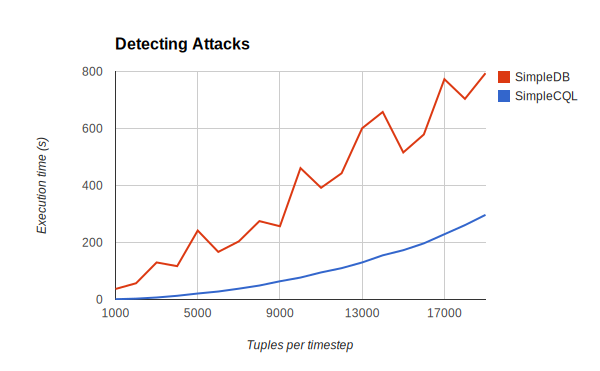
\includegraphics[totalheight=5cm]{attack.png}}
    \caption{Performance of SimpleDB and SimpleCQL detecting attacks.}
    \label{fig:attack}
\end{figure}

As shown in Figure~\ref{fig:attack}, SimpleCQL was able to drastically outperform SimpleDB.

\subsection{Trending Tweets}
Trending tweets on Twitter are useful for a variety of reasons.  The company may use them to increase user engagements, optimize advertisements, or analyze the state of current events.  

In this example, we consider a stream of Twitter tweets, \texttt{TweetStream}. We formally define the schema of the stream as: \texttt{TweetStream\{Text:STRING, Hashtag:STRING, Location:STRING\}}.  Given this schema, a rolling count of log messages that contain the string “failed login” provides the relevant information for the above situation.  The following query computes the rolling count.

\begin{verbatim}
SELECT ISTREAM(
    TweetStream.Hashtag,
    MAX(COUNT(*))
)
FROM TweetStream [Range 30 seconds]
WHERE TweetStream.Location = ‘Boston’
GROUP BY TweetStream.Hashtag;
\end{verbatim}


Data for the \texttt{TweetStream} was generated prior to running tests.  The data generated represents 30 minutes of tweets with text, hashtags, and locations.  

\begin{figure}[tpH!]
    \centering
    \centerline{\includegraphics[totalheight=5cm]{trending.png}}
    \caption{Performance of SimpleDB and SimpleCQL calculating trending tweets.}
    \label{fig:attack}
\end{figure}

\subsection{Advertisement Statistics}
The Advertising Statistics example, presented in detail in section 2, involves joining advertisement insertions across two disparate streams.  Specifically a stream of advertisement insertions, known as \texttt{InsertionStream}, and a stream of advertisement events, known as \texttt{EventStream}, are joined on \texttt{InsertionId} in order product real-time per-advertisement click-through rate.  The following query computes the join.

\begin{verbatim}
SELECT RSTREAM (
    advertisement_id,
    SUM(type = 'click' ? 1 : 0) / 
    SUM(type = 'impression' ? 1 : 0)
)
FROM (
    SELECT ISTREAM(advertisement_id, type)
    FROM InsertStream [Range 600 seconds], 
         EventStream [Range 1 second] 
    WHERE InsertStream.insertion_id = 
    EventStream.insertion_id
) 
GROUP BY advertisement_id;
\end{verbatim}

Data for the \texttt{InsertionStream} and \texttt{EventStream} was generated prior to running tests.  The data generated represents 30 minutes of advertisement insertions.  Each insertion in the \texttt{InsertionStream} may have a corresponding impression and click event in the EventStream that appears up to 10 minutes after the insertion.

\begin{figure}[tpH!]
    \centering
    \centerline{\includegraphics[totalheight=5cm]{ads.png}}
    \caption{Performance of SimpleDB and SimpleCQL calculating real time CTR.}
    \label{fig:attack}
\end{figure}

\subsection{Garbage collection}
As expected Garbage collection drastically reduced the memory footprint of the system, but reduced performance slightly. These points are better illustrated in the following graphs.


\bibliographystyle{plain}
\bibliography{references}


\end{document}
